\subsection{Vertical Advective Velocity and Reference Diffusivity}
\label{sec:AdvVelDiffCoeff}

Transport out of the \gls{EBS} and through the permeable, porous geosphere 
involves advection, diffusion, and hydraulic dispersion phenomena. Advection is 
transport driven by bulk water velocity, while diffusion is the result of 
Brownian motion across concentration gradients.  The method by which the 
dominant solute transport mode (diffusive or advective) is determined for a 
particular porous medium is by use of the dimensionless Peclet number, 

\begin{align} 
  Pe &= \frac{nvL}{\alpha \theta v + D_{eff}},\\
  &= \frac{\mbox{advective rate}}{\mbox{diffusive rate}}\nonumber
  \intertext{where} 
  \theta &= \mbox{ solute accessible porosity } [\%]\nonumber\\
  v &= \mbox{ advective velocity } [m\cdot s^{-1}] \nonumber\\
  L &= \mbox{ transport distance } [m]\nonumber\\
  \alpha &= \mbox{ dispersivity } [m]\nonumber\\
  D_{eff} &= \mbox{ effective diffusion coefficient } [m^2\cdot s^{-1}].\nonumber
\end{align}

For a high $Pe$ number, advection is the dominant transport mode, while 
diffusive or dispersive transport dominates for a low $Pe$ number
\cite{schwartz_fundamentals_2004}.

In this analysis, the threshold between primarily diffusive and primarily 
advective transport was investigated by varying the vertical advective velocity 
in conjunciton with the diffusion coefficient.  It was expected that for the low 
diffusion coefficients and low advective velocities usually found in clay media, 
the model should behave entirely in the diffusive regime, but as the 
vertical advective velocity grows, system behavior should 
increasingly approach the advective regime. 


\subsubsection{Parametric Range}

The diffusion coefficient was altered as in Section \ref{sec:diffusivity} and 
the vertical advective velocity of the far field was altered as well.

From Table 5.5-1 of the Argile Safety Evaluation by \gls{ANDRA}, the vertical 
hydraulic gradient is $0.4$, while the hydraulic conductivity is $5.0\times10^{14} 
[m/s]$. The resulting vertical advective velocity is then $2.0\times10^{-14}[m/s]$, which is 
$6.31\times10^{-7}[m/yr]$  \cite{andra_argile:_2005}. %9


As in Section \ref{sec:diffusivity}, in order to isolate the effect of the far 
field behavior, the waste form degradation rate was set to be very high as were 
the solubility and advective flow rate through the  \gls{EBS}. This guarunteed 
that in the first few time steps, the far field was the primary barrier to 
release. 

The forty runs are a combination of the five values of the vertical advective 
velocity and eight magnitudes of relative diffusivity (see Table 
\ref{tab:AdvVelAndDiffCoeffGroups}). 

\begin{table}[hbp!]
\centering
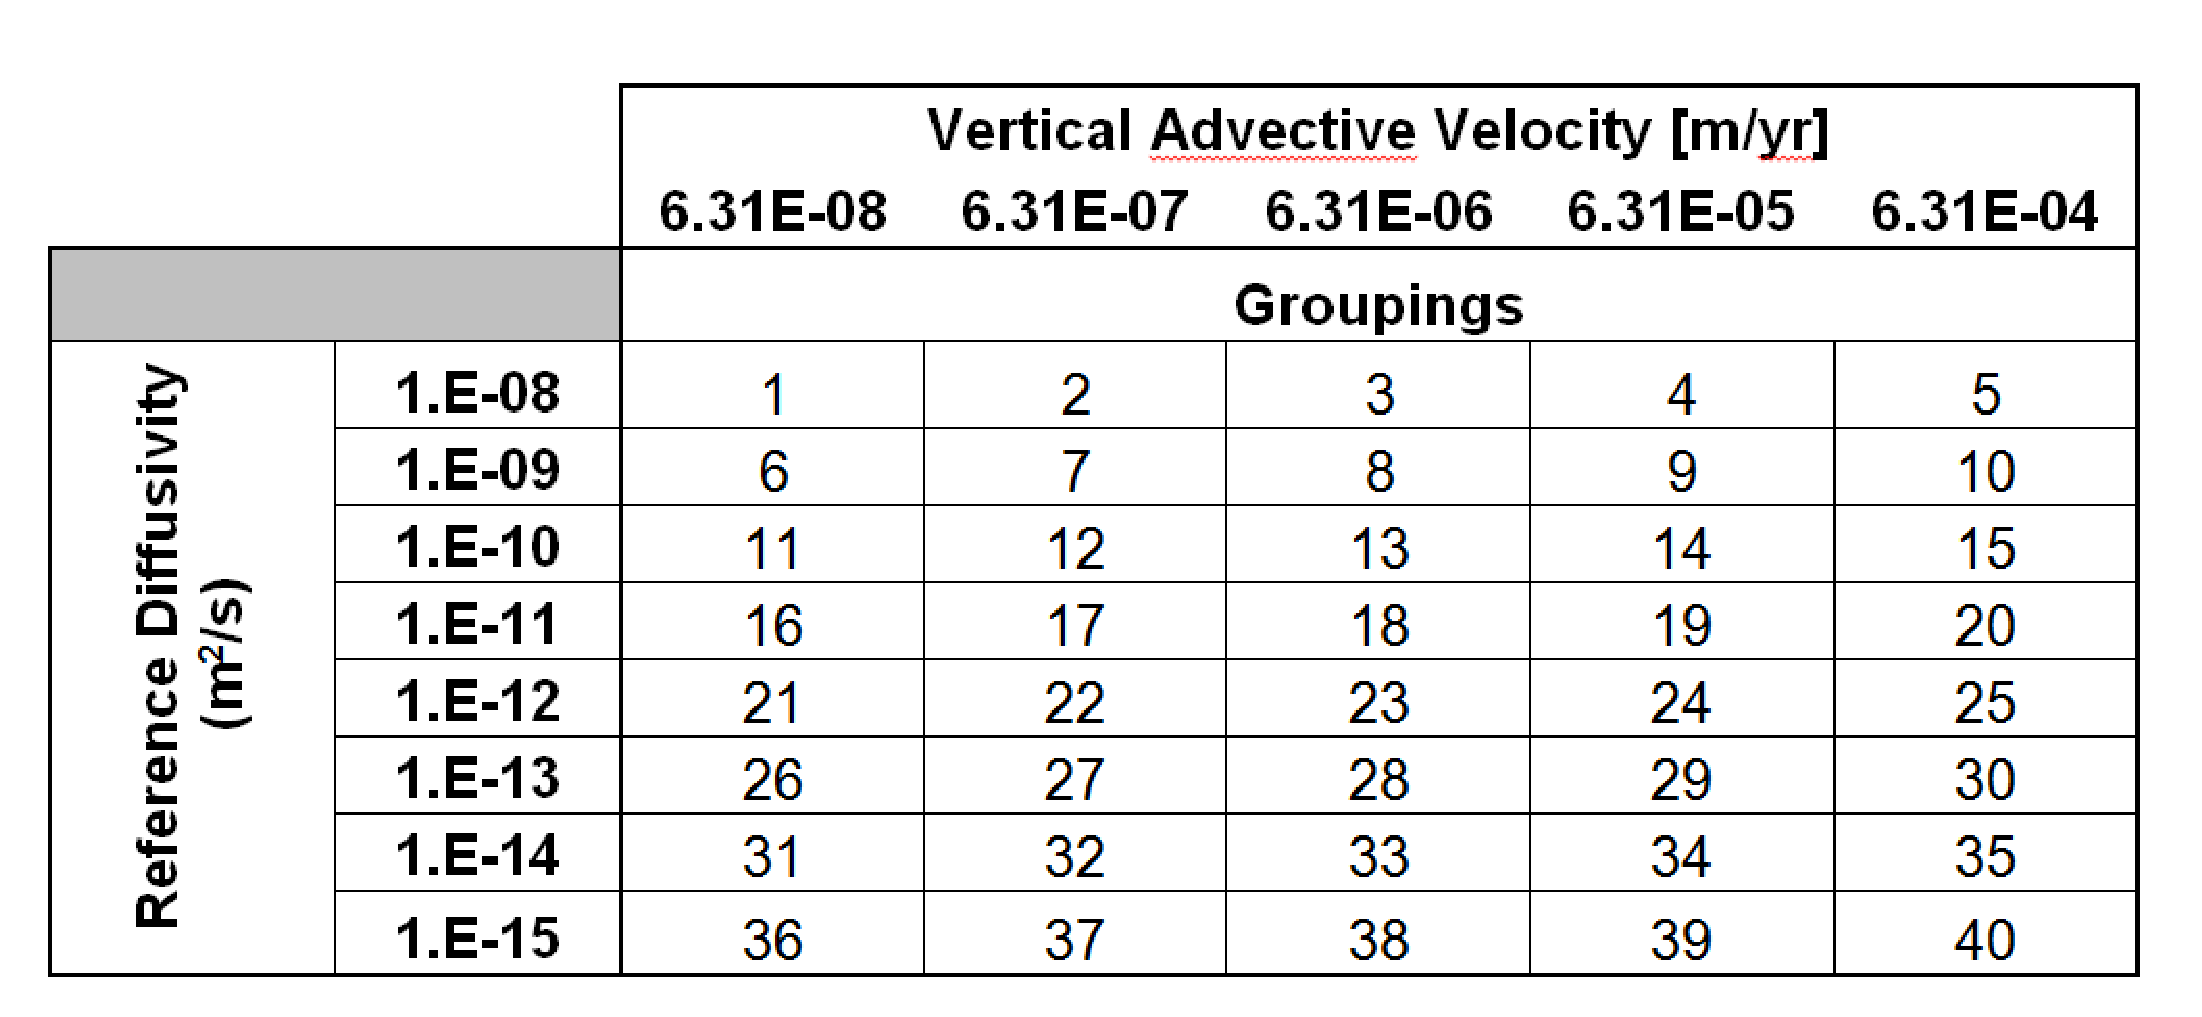
\includegraphics[width=0.7\textwidth]{./chapters/nuclide_sensitivity/clay/AdvVelAndDiffCoeffEBSFail/AdvVelAndDiffCoeffGroups.eps}
\caption{Vertical advective velocity and diffusion coefficient simulation groupings.}
\label{tab:AdvVelAndDiffCoeffGroups}
\end{table}


To capture the importance of the vertical advective velocity, a range was chosen 
to span a number of orders of magnitude between $ 6.31\times 10^{-8}$ 
and $ 6.31\times10^{-4} [m/yr]$. The relative diffusivity was simultaneously varied 
over the eight magnitudes between $ 10^{-8}$ and $ 10^{-15} [m^2/s]$. It is 
worth noting that both the relative diffusivity and the vertical advective 
velocity are functions of porosity in the host rock and are therefore expected 
to vary together. 

%Importantly, the thermal fluxes near the waste have an impact on the dynamic 
%viscosity of the hydraulic medium and can be expected to triple the vertical 
%advective velocity within a clay repository during the heating period 
%\cite{andra_argile:_2005}. %pg 429




